% Inline licence here

\documentclass[a4paper,12pt]{report}

% Include Packages
\usepackage[a4paper,left=2.5cm,top=2.5cm,bottom=2.5cm,
	right=2.5cm]{geometry}
\usepackage{url}
\usepackage{fancyhdr}
\usepackage{titlesec}
\usepackage{graphicx}
\graphicspath{ {images/} }

%=============Formating============%
% Customize chapter 
\titleformat{\chapter}[block]{\LARGE\bfseries}{Chapter \thechapter}
{0.5em} % sep
{} % before-code
[] % after-code

% Page Header and Footer
\pagestyle{fancy}
\rhead{\textbf{Enhance ManageIQ}}
\chead{}
\lhead{}
\lfoot{Department of Computer Science and Engineering. RIT,Rajaramnagar}
\cfoot{}
\rfoot{\thepage}
\renewcommand{\footrulewidth}{.4pt}
\renewcommand{\headrulewidth}{.4pt}


% Redefine for plain styling page
\fancypagestyle{plain}{
\rhead{}
\chead{}
\lhead{}
\lfoot{Department of Computer Science and Engineering. RIT,Rajaramnagar}
\cfoot{}
\rfoot{\thepage}
\renewcommand{\headrulewidth}{0pt}
\renewcommand{\footrulewidth}{.4pt}
}


%% To check font size %%
\makeatletter
\newcommand{\showfontsize}{\f@size{} pt}
\makeatother

\begin{document}
\tableofcontents{}

\chapter{Introduction}
Cloud is a buzzword in today's world as cloud is used by a person every time , any time, anywhere and anyhow. Cloud is the solution to any storage or computational work. Cloud is a huge platform to explore and yet lot to learn. Cloud management means the software and technologies designed for operating and monitoring applications, data and services residing in the cloud. Cloud management tools help ensure cloud computing-based resources are working optimally and properly interacting with users and other services.\\

Cloud management strategies typically involve numerous tasks including performance monitoring, security and compliance auditing and management, and initiating and overseeing disaster recovery and contingency plans.\\

Public cloud is one based on the standard cloud computing model, in which a service provider makes resources, such as virtual machines (VMs), applications or storage, available to the general public over the internet. Public cloud services may be free or offered on a pay-per-usage model.\\

Private cloud is a type of cloud computing that delivers similar advantages to public cloud, including scalability and self-service, but through a proprietary architecture. Unlike public clouds, which deliver services to multiple organizations, a private cloud is dedicated to a single organization.\\

Hybrid cloud is maintained by both internal and external providers. In effect, a hybrid cloud is a combination of public and private cloud services, with orchestration between the two. In some cases, this model is attractive because it enables organizations to tap into the benefits of the public cloud, while maintaining their own private cloud for sensitive, critical or highly regulated data and applications.\\

ManageIQ is an open source management platform for Hybrid IT. It can manage small and large environments, and supports multiple technologies such as virtual machines, public clouds and containers.

With ManageIQ you will be able to:
\begin{itemize}
	\item Continuously discover the latest state of your environment.
	\item Implement self service for your end users.
	\item Enforce compliance across the environment.
	\item Optimize the performance and utilization of your environment.
\end{itemize}

Virtualization is the creation of a virtual rather than actual version of something, such as an operating system, a server, a storage device or network resources.\\

Operating system virtualization is the use of software to allow a piece of hardware to run multiple operating system images at the same time. The technology got its start on mainframes decades ago, allowing administrators to avoid wasting expensive processing power.\\

Cloud Providers serve different purposes and services. Some of the cloud providers are mentioned  below.\\

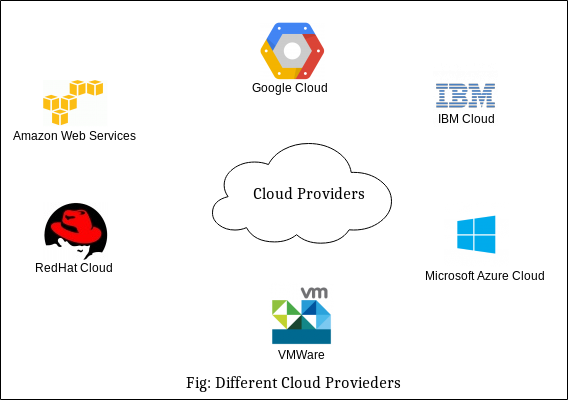
\includegraphics[scale=.75]{cloud_providers}

\chapter{Problem Statement}
ManageIQ is an open source cloud management platform. It was founded by Red Hat as a community project in 2014, and forms the basis for its CloudForms product. It allows centralized management of various virtualization, private cloud, public cloud, containers, middleware and software defined networking technologies.\\

ManageIQ is written in the Ruby language and uses the Ruby on Rails framework. The ManageIQ software is shipped as a pre-built virtual appliance, roughly 1GB in size. The appliance is based on the CentOS operating system, and includes an embedded PostgreSQL database. Since the Darga release, a container based version has also been made available.\\

Fine is the latest release of ManageIQ on 17 May 2017 which mainly focuses on automation with Ansible, improved AWS support including storage, new Physical Infrastructure provider type.\\

Ansible is an open source automation platform. Ansible can help you with configuration management, application deployment, task automation. In simple terms assume you need to install a thing suppose tomcat on different systems, usually admin will have to install separately on those different machines. But now with the latest technologies you can do this task easier using ansible. Admin will assign this task to a machine, and whenever tomcat needs to be installed the machine will install the instance for it rather than admin and will be easier. For this they need two things, Inventory Files and Playbook.\\

Playbook contains a number of plays in it while plays have different tasks within them. These tasks call the module. All the tasks in a play run sequentially and they as well trigger the handlers that are run once at the end of the play. Handlers are itself a task. The plays in playbook and the tasks in the play can also be from different other playbooks.\\

Since ManageIQ code-name Fine release it is possible to automate environment using Ansible instead of ManageIQ's legacy Automate Datastore which uses Ruby. \textbf{Goal of this project is to develop automation using Ansible and Ruby to extend usage of ManageIQ for hybrid cloud management and automation.}


\chapter{Literature Survey}

Linux is a name which broadly denotes a family of free and open-source software operating system distributions built around the Linux kernel. The defining component of a Linux distribution is the Linux kernel, an operating system kernel first released on September 17, 1991 by Linus Torvalds.\\

Typically, Linux is packaged in a form known as a Linux distribution for both desktop and server use. Some of the most popular and mainstream Linux distributions are Arch Linux, CentOS, Debian, Fedora, Gentoo Linux, Linux Mint, Mageia, openSUSE and Ubuntu, together with commercial distributions such as Red Hat Enterprise Linux and SUSE Linux Enterprise Server.\\

In many ways, Linux is similar to other operating systems you may have used before, such as Windows, OS X, or iOS. But Linux also is different from other operating systems in many important ways. First, and perhaps most importantly, Linux is open source software. The code used to create Linux is free and available to the public to view, edit, and—for users with the appropriate skills—to contribute to.\\

Linux is also different in that, although the core pieces of the Linux operating system are generally common, there are many distributions of Linux, which include different software options. This means that Linux is incredibly customizable, because not just applications, such as word processors and web browsers, can be swapped out.\\

Git is a free and open source distributed version control system designed to handle everything from small to very large projects with speed and efficiency. Git was created by Linus Torvalds in 2005 for development of the Linux kernel, with other kernel developers contributing to its initial development. 2.15 is the latest git version released on 2017-10-30.\\

Virtualization is technology that allows you to create multiple simulated environments or dedicated resources from a single, physical hardware system. Software called a hypervisor connects directly to that hardware and allows you to split 1 system into separate, distinct, and secure environments known as virtual machines (VMs). These VMs rely on the hypervisor’s ability to separate the machine’s resources from the hardware and distribute them appropriately.\\

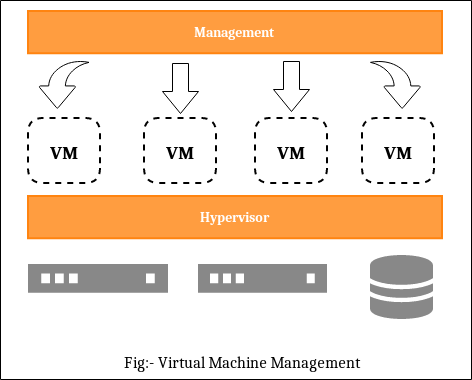
\includegraphics[scale=.85]{vm_management}\\

Types of virtualization:
\begin{itemize}
	\item Server Virtualization
	\item OS Virtualization
	\item Network Virtualization
	\item Hardware Virtualization
	\item Application Virtualization
	\item Storage Virtualization
\end{itemize}

Ruby is a dynamic, reflective, object-oriented, general-purpose programming language. It was designed and developed in the mid-1990s by Yukihiro "Matz" Matsumoto in Japan. According to its creator, Ruby was influenced by Perl, Smalltalk, Eiffel, Ada, and Lisp. It supports multiple programming paradigms, including functional, object-oriented, and imperative. It also has a dynamic type system and automatic memory management. 2.4 is the latest ruby version with 2.4.2 as latest tenant on date 2016-12-25 and hoping for 2.5 version of ruby in Dec'17. The syntax of Ruby is broadly similar to that of Perl and Python.\\

OpenStack is a free and open-source software platform for cloud computing, mostly deployed as infrastructure-as-a-service (IaaS), whereby virtual servers and other resources are made available to customers. OpenStack Pike is latest version of OpenStack released on 30 August 17. The goals of the OpenStack initiative are to support interoperability between cloud services and allow businesses to build Amazon-like cloud services in their own data centers.\\

Cloud computing has made drastic change in the reduction of hardware and software cost and other server resources as well.Cloud computing solutions for business leads to increased efficiency; services are rapidly deployed and ready for use in minutes.\\

As we know public and private cloud are used by different organizations, colleges, universities, etc. Private cloud provides scalability, elasticity, self service, etc. but to a single organization where the security is measured. Public cloud is same as private but shared among different organizations where security can be at risk. Whereas hybrid cloud is the combination of the two different clouds i.e. Public as well Private cloud. \\

With cloud automation, an organization eliminates these repetitive and manual processes for workload deployment and management. To achieve cloud automation, an IT team needs to use orchestration and automation tools that run on top of their virtualized environment. Orchestration enables an administrator to codify the various steps and processes involved with workload deployment and management, while automation invokes those steps without human intervention.So we thought of automating hybrid cloud using Ansible and Ruby to enhance its use with ManageIQ. This will help increase the use and enhancement of hybrid cloud.\\

\chapter{National/International Status}

Since 2000, cloud computing has come into existence. In early 2008, NASA's OpenNebula, enhanced in the RESERVOIR European Commission-funded project, became the first open-source software for deploying private and hybrid clouds, and for the federation of clouds. In the same year, efforts were focused on providing quality of service guarantees (as required by real-time interactive applications) to cloud-based infrastructures, in the framework of IRMOS European Commission-funded project, resulting in a real-time cloud environment.\\

In August 2006 Amazon introduced its Elastic Compute Cloud. Microsoft Azure was announced as "Azure" in October 2008 and was released on 1 February 2010 as Windows Azure, before being renamed to Microsoft Azure on 25 March 2014.\\

In July 2010, Rackspace Hosting and NASA jointly launched an open-source cloud-software initiative known as OpenStack. The OpenStack project intended to help organisations offering cloud-computing services running on standard hardware. The early code came from NASA's Nebula platform as well as from Rackspace's Cloud Files platform. As an open source offering and along with other open-source solutions such as CloudStack, Ganeti and OpenNebula, it has attracted attention by several key communities. Several studies aim at comparing these open sources offerings based on a set of criteria.\\
s
On June 19,2014, Red Hat Inc., the world’s leading provider of open source solutions, announced the launch of the ManageIQ community with the availability of ManageIQ’s fully open-sourced code repository and the first builds of the project. The ManageIQ community aims to provide the industry's leading open source cloud management platform with advanced governance and automation capabilities.
"With the full release of the ManageIQ code, Red Hat is making an important contribution towards the development of an open cloud management ecosystem"
\footnote{Mary Johnston Turner, Research Vice President, Enterprise Systems Management Software, IDC Research}\\

ManageIQ community announced Fine Beta release of ManageIQ on April 5,2017. Fine is the next milestone release for ManageIQ cloud and virtualization management platform. With each release, ManageIQ gets more robust and feature complete across providers. In this release, a lot of attention was given to Ansible. However, other providers, REST API, as well as performance also benefit in this release.\\

Red Hat CloudForms is an enterprise grade cloud management platform, sold by Red Hat to its customers under a subscription model. CloudForms is based on code from the open source ManageIQ project.

\chapter{Applications}
ManageIQ is used for management of hybrid cloud. Cloud management is the management of cloud computing products and services. Public clouds are managed by public cloud service providers, which include the public cloud environment’s servers, storage, networking and data center operations. Managing a private cloud requires software tools to help create a virtualized pool of compute resources, provide a self-service portal for end users and handle security, resource allocation, tracking and billing.\\

In hybrid cloud environments, compute, network and storage resources must be managed across multiple domains, so a good management strategy should start by defining what needs to be managed, and where and how to do it.\\

Network management is the process of administering and managing the computer networks of one or many organisations. Various services provided by network managers include fault analysis, performance management, provisioning of network and network devices, maintaining the quality of service, and so on. Software that enables network administrators or network managers to perform their functions is called network management software.\\

Cloud management is the management of cloud computing products and services. Public clouds are managed by public cloud service providers, which include the public cloud environment’s servers, storage, networking and data center operations. Managing a private cloud requires software tools to help create a virtualized pool of compute resources, provide a self-service portal for end users and handle security, resource allocation, tracking and billing.\\

In hybrid cloud environments, compute, network and storage resources must be managed across multiple domains, so a good management strategy should start by defining what needs to be managed, and where and how to do it.\\

Cloud computing is an information technology (IT) paradigm, a model for enabling ubiquitous access to shared pools of configurable resources (such as computer networks, servers, storage, applications and services), which can be rapidly provisioned with minimal management effort, often over the Internet. Cloud computing allows users and enterprises with various computing capabilities to store and process data either in a privately-owned cloud, or on a third-party server located in a data center, thus making data-accessing mechanisms more efficient and reliable.\\

Storage management usually refers to the management of Computer data storage, which includes memory management. It can also refer to specific methods or products for storage management, such as the following
\begin{itemize}
	\item ADSTAR Distributed Storage Manager
	\item Automatic Storage Management
	\item Hierarchical storage management
	\item IBM Tivoli Storage Manager
	\item OpenView Storage Area Manager
	\item Storage Management Initiative - Specification
	\item Storage Resource Manager
	\item Storage Resource Management
\end{itemize}

Cloud automation is a fundamental building block for the cloud computing paradigm. Automation aims to make all activities related to cloud computing as fast, efficient, and as hands off as possible through the use of various software automation tools which are installed directly on the virtualization platform or software and controlled via an intuitive interface.\\

Cloud Optimization is about automating and refining the standardization of your infrastructure. It is also about taking advantage of the unique characteristics of the cloud. Companies at this stage have a holistic business view of the cloud ecosystem, with tools that facilitate optimization, standardization, and reporting from a business perspective. Organizations at the optimization phase are trying to utilize as close to 100% of the resources provisioned as possible while maintaining availability and performance across their workloads.


\chapter{Objectives of Project}
\begin{enumerate}
	\item Understand basic concepts required for project
	\item Create project environment and deploy ManageIQ appliance
	\item Setup and configuration of ManageIQ 
	\item Setup provider and integrate 	this provider with ManageIQ
	\item Review Provider details 
	\item Provision instance form ManageIQ
	\item Develop Ansible Playbooks which can be imported as ansible repositories in ManageIQ.
	\item Develop Service dialogs needed to execute playbooks as service catalogs
	\item Develop or/and enhance code required for automate
	\item Write documentation which should help others to use those playbooks in their environment
\end{enumerate}

\chapter{Future Scope}
Adoption of cloud computing technology has significantly increased over the last few years, promising a great opportunity for innovation amongst businesses. However some businesses are still sceptical of how Cloud Computing can enhance or replace all or part of their IT environment.\\

Cloud is typically marketed to promote benefits such as improved efficiency, flexibility and even opportunity for expansion. However many of these benefits lack tangibility, often making it difficult to validate a move to the cloud.\\

Organisations considering the change typically look at implementing a solution that incorporates a mix of on premise, and public or private cloud, referred to as a hybrid cloud model.\\

Business continuity has been identified as one of the most important elements of business operations. A business continuity solution is not just simply backing up and/or replicating content to the cloud, nor is it simply a Disaster Recovery plan. Business continuity is to continue to do business during a failure or disaster. In basic terms, it means that when a failure or disaster happens, that data is still accessible with little to no downtime.\\

A business continuity solution therefore needs to be planned to consider key elements such as resilience, recovery and contingency. Hybrid cloud solutions are often considered by organisations as a key component of a business continuity solution where critical data is replicated to a cloud solution in a different location to the primary systems. This provides data insurance in the event of a disaster (natural or technological), minimising downtime and the costs associated with such an event. Understanding this benefit, service providers have streamlined their offerings to easily integrate a business continuity solution into hybrid cloud systems.\\

Barriers to innovation are reduced in a cloud environment, as large capital expenditure is not required for modelling a new service. Previously, cost associated with such a task would include capital expenditure for infrastructure, labour and time for research then more resources to install and maintain. This places a lot of pressure on capacity management practices and perfect forecasting despite many uncertain variables. In hybrid cloud, concepts can be tested without capital expenditure, prototyped in a cloud environment then rapidly deployed and measured for success. The added benefit of hybrid cloud is the availability of resources combining both internal and external environments including data, network, and infrastructure, all available on iseek’s cloud environment.\\

Scaling on IT infrastructure can be extremely expensive, inefficient and places much more pressure on accurate forecasting in growing companies. However, a hybrid cloud environment can provide the opportunity for businesses to scale out to a cloud environment for specific workloads. Implementing automation rules on the cloud provides the ability to scale resources up and down as business demands change. This allows the hybrid cloud system to take advantage of unlimited resources based on demand driven usage, optimising the environment for performance and efficiency.\\

In many organisations, speed to market is a key differentiator. In a digital age, the ability to quickly spin up environments to test, prototype and launch new products is highly desirable. For organisations with an IT infrastructure that is working near or close to capacity, spinning up a new environments can become a challenge and potentially hinder the business\\

Hybrid cloud allows resources to be deployed and commissioned in an automated process that can yield results at hugely improved speeds, so companies are no longer limited by their IT footprint.\\

Companies can leverage hybrid cloud as the first step in moving to a predominately cloud environment. A hybrid solution provides the perfect opportunity for companies to test the capability of certain workloads and providers in a cloud based environment and assist them in planning their cloud strategy. However planning is key, as hybrid cloud can require complex design to coherently combine an organisation’s platform with a cloud environment.

\chapter{Methodology}

\textbf{Setup project environment}\\
The virtual machine requires 8Gb RAM and four vCPU to run ManageIQ fluently. The system is installed using CentOS operating system. CentOS is a linux flavour with linux kernel.\\

\textbf{ManageIQ installation on Virtual Machine}\\
ManageIQ appliance is required for this which can be run on QEMU/KVM. ManageIQ appliance is directly available on the ManageIQ site. So this qcow2 image is to be downloaded and deploy it on VM. After launching instance of that VM, we are able to run ManageIQ service. The ManageIQ applicancation can be controlled using appliance-console with command line interface.\\

\textbf{OpenStack installation using packstack}\\
OpenStack is installed on the machine using packstack to manage the controlling and monitoring of the private cloud. We need to install OpenStack allinone installation and configure to launch instances. Integration of OpenStack in ManageIQ in required to monitor the instances and services of OpenStack.\\

\textbf{Develop Ansible Playbook}\\
Installation on Ansible and develop playbook which can be imported in ManageIQ for automation. Learn to develop playbook is required.\\

\textbf{Create service dialogs}\\
Dialog services are needed to be created to execute the above created ansible playbook.\\

\textbf{Create documentation}\\
Doing a task is must, but its documentation is more valuable as that of project. The details of the projects are to be documented with all the installation procedure and the actual flow of project implementation to help other people understand the project brightly.\\

\chapter{Conclusion}

ManageIQ is a platform for manage, control and optimize cloud. It can manage small and large environments, and supports multiple technologies such as virtual machines, public clouds and containers.\\

A cloud operating system that controls large pools of compute, storage, and networking resources throughout a data center, all managed through a dashboard that gives administrators control while empowering their users to provision resources through a web interface. OpenStack is an open source project licensed under the Apache License 2.0.\\
    
Installation of ManageIQ platform on virtual machine is done successfully. OpenStack installation is accompanied with this. Hoping forward to complete all the tasks successfully. Automation will help system administrator to manage the cloud efficiently with cost optimization. This can minimize the recursive work. Ansible is a emerging platform to automate things which is very popular because of its simplicity.

\chapter{References}
\begin{enumerate}
	\item Project Link
	
	https://github.com/psachin/projects/blob/manageiq-ansible-playbook/manageiq-ansible-playbook.md
	
	\item ManageIQ Documentation
	
	http://manageiq.org/docs/
	
	\item RDO Packstack Installation
	
	https://www.rdoproject.org/install/packstack/
	
	
\end{enumerate}
\end{document}

